\subsection{L'ancien processus de la maintenance}
La première version du module de la maintenance ne prend en compte que les analyseurs 
(automates) dans un laboratoire. Étant limité aux analyseurs, ce module ne répond plus
 aux besoins des laboratoires.
L’informatisation des processus d’analyses médicales a engendré de nouveaux besoins qui 
s’interconnectent.
Aujourd’hui, de nouveaux équipements rentrent en jeu dans la procédure 
d’analyses médicales tels que les imprimantes, les scanners, les microscopes, 
les équipements informatiques, etc.
\begin{figure}[hp]
    \centering
    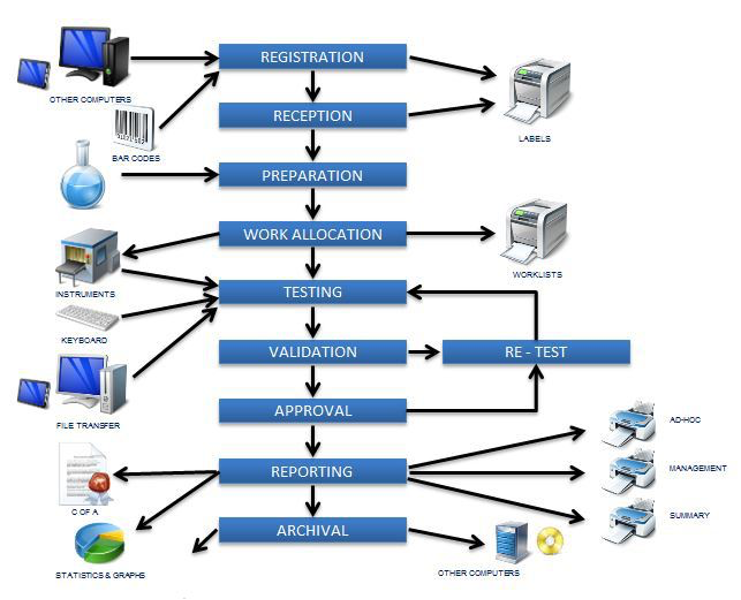
\includegraphics[width=400pt,height=400pt]{images/processus_old.png}
    \caption{Workflow de laboratoire}
\end{figure}

Le schéma précèdent montre que dans un workflow de laboratoire d’analyses médicales, 
plusieurs équipements médicaux et non-médicaux sont nécessaires pour assurer le bon 
déroulement de ce dernier. 
À l’instar des analyseurs, tous ces équipements demandent un entretien particulier 
pour assurer leur fonctionnement, la sureté de leurs résultats ainsi que leurs 
disponibilités en permanence. 
\pagebreak

C’est pour cette raison que l’évolution du module de la maintenance devient 
une nécessité pour l’équipe technique de Clarisys Informatique. Avec ce module MCA, 
elle peut gérer d’une manière plus générale les opérations de maintenance concernant 
les équipements auxquels il se connecte.
Actuellement, si nous voulons planifier une opération de maintenance pour un analyseur, 
nous pouvons nous rendre à l’interface de planifications de maintenances dans le menu de
 paramétrages de MCA.

Anciennement, si nous voulons planifier une opération de maintenance pour un analyseur, 
nous pouvons nous rendre à l’interface de planifications de maintenances dans le menu 
de paramétrages de MCA.
\begin{figure}[hp]
    \centering
    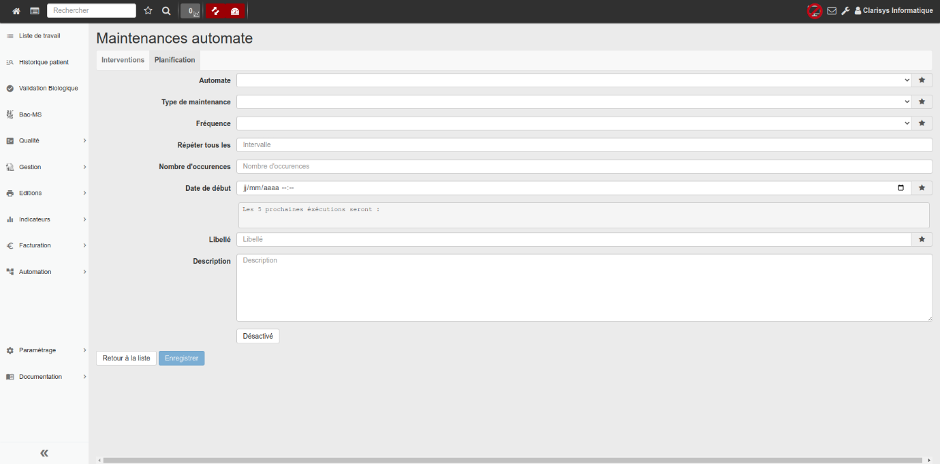
\includegraphics{images/old_interface_maint.png}
    \caption{L'incienne interface de paramétrage de maintenances - MCA}
\end{figure}

Cette interface, ne permet pas à l’agent de maintenance de consulter les informations 
concernant les analyseurs telles que leurs marques, leurs fournisseurs, leurs contrats 
de prestations, le contact de l’entreprise de maintenance si prestation externe, etc.
De plus, aucune information concernant l’état de l’analyseur n’est consultable. 
Par exemple : la date de la dernière intervention de maintenance faite sur l’analyseur, 
les interventions à venir et leurs dates, les interventions précédentes et leurs 
informations.
Ces informations sont très importantes pour établir ce que l’on appelle le registre 
de vie ou le cahier de vie d’analyseur, dans lequel, on retrouve les registres ou 
grilles de maintenances mis à jour par les techniciens de maintenances.

En conclusion, une évolution de ce module permet, d’une part, de mieux comprendre 
le fonctionnement du laboratoire d’analyses médicales et d’autre part d’aider les 
agents de maintenance à organiser les opérations de maintenance non seulement 
pour les automates mais pour tout type d’équipements de laboratoire.
\pagebreak